\documentclass{article}
\usepackage[utf8]{inputenc}

\usepackage{amsmath, amssymb, amsthm}
\usepackage{enumitem}
\usepackage{hyperref}
\usepackage{float}
\usepackage{tikz}

\usepackage{listings}
\usepackage{xcolor}

\definecolor{codegreen}{rgb}{0,0.6,0}
\definecolor{codegray}{rgb}{0.5,0.5,0.5}
\definecolor{codepurple}{rgb}{0.58,0,0.82}
\definecolor{backcolour}{rgb}{0.95,0.95,0.92}

\lstdefinestyle{thestyle}{
    backgroundcolor=\color{backcolour},
    basicstyle=\ttfamily\footnotesize,
    keywordstyle=\color{red!80}\bfseries,
    ndkeywordstyle=\color{blue!80}\bfseries,
    identifierstyle=\color{black},
    commentstyle=\color{codegreen},
    stringstyle=\color{codepurple},
    breakatwhitespace=false,
    breaklines=true,
    captionpos=b,
    keepspaces=true,
    numberstyle=\tiny\color{codegray},
    numbers=left,
    numbersep=2pt,
    showspaces=false,
    showstringspaces=false,
    showtabs=false,          
    tabsize=2
}

\lstset{style=thestyle}

\lstdefinelanguage{TML}{ 
    keywords={changeto, move, goto, if, switch, while, module, accept, reject, halt, alphabet},
    ndkeywords={left, right, tapehead, blank},
    sensitive=true,
    comment=[l]{//},
    morecomment=[s]{/*}{*/},
    morestring=[b]',
    morestring=[b]"
}

\newtheorem{theorem}{Theorem}[section]
\theoremstyle{definition}
\newtheorem{definition}[theorem]{Definition}
\newtheorem{remark}[theorem]{Remark}
\newtheorem{example}[theorem]{Example}

\title{TML Equivalence Proof}
\author{Pete Gautam}

\begin{document}
    \maketitle

    \begin{abstract}
        This document proves the equivalence of the TML with TMs. We do this by constructing an equivalent TML program for a TM, and vice versa. In the first section, we define complete TML programs, which are very close to TMs, and describe how they can be mapped into TMs. 
    \end{abstract}

    \section{Complete TML programs}
    \noindent Complete programs in the TML are a specific type of TML programs that are very detailed and obey different properties. As such, it is very easy to construct the TM corresponding to a complete program. In this section, we will build to the definition complete programs from complete blocks and modules.
    \begin{definition}
        Let $P$ be a valid TML program, and let $B$ be a basic block in $P$. We say that $B$ is a \emph{complete block} if it is composed of all the 3 commands: a \textit{changeto} command, a \textit{move} command, and a \textit{flow} command. If the \textit{flow} command is missing, we say that $B$ is a \emph{partially complete block}.
    \end{definition}

    Complete blocks contain all the information required to transition from one state to another. This is because of the following:
    \begin{itemize}
        \item A complete block lists the next value of the tapehead; we assume the original value of the tapehead to be known outwith the block.
        \item A complete block states which direction the tapehead is moving- left or right.
        \item A complete block determines precisely what the next state is for the block- it is either a terminating state or we are going to the initial block of another module.
    \end{itemize}        
    We can convert any basic block with a \textit{flow} command to a complete block by adding the default commands (i.e. moving left and changing the tapehead value to the current value). Equally, it is quite straightforward to convert a complete block into a subpart of a Turing Machine.
    \begin{example}
        Consider the following complete block.
\begin{lstlisting}[language=TML]
changeto a
move right
goto s2
\end{lstlisting}
        \noindent If we are at the state $s_1$, and the block applies when the tapehead value is $b$, then the following is the corresponding subpart of the Turing Machine:
        \begin{figure}[H]
            \centering
            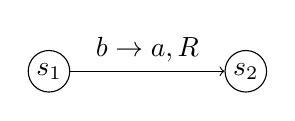
\begin{tikzpicture}
                \node[circle, draw=black, fill=white, inner sep=0pt, minimum size=15pt] (s1) at (0, 0) {$s_1$};
                \node[circle, draw=black, fill=white, inner sep=0pt, minimum size=15pt] (s2) at (2.5, 0) {$s_2$};
    
                \draw[->] (s1) -- node[above] {$b \to a, R$} (s2);
            \end{tikzpicture}
            \caption{The TM subpart of the given Turing Machine complete block.}
        \end{figure}            
    \end{example}
    
    Using complete and partially complete blocks, we can define complete modules.
    \begin{definition}
        Let $P$ be a valid TML program, and let $M$ be a module in $P$. We say that $M$ is a \emph{complete module} if all of the following hold:
        \begin{itemize}
            \item it is composed of a single switch block;
            \item the body of each \textit{if} command is a complete block; and
            \item the body of each \textit{while} command is a partially complete block.
        \end{itemize}
    \end{definition}
    % \begin{remark}
    %     Having no \textit{if} commands in a complete module means that the Turing machine never terminates. This is not an issue since it is still a valid Turing machine. 
    % \end{remark}
    \begin{remark}
        For a \textit{while} command, the body must be partially complete because the corresponding edge in the TM is always a loop.
    \end{remark}
    It is quite easy to map a single module to a sub-Turing machine. It precisely corresponds to having an initial state and edges going to other states as dictated by each case. Because the program is valid, we know that there is a case for each letter in the alphabet, including the \texttt{blank} letter.
    \begin{example}
        Consider the following complete module.
\begin{lstlisting}[language=TML]
module basic {
    switch tapehead {
        while b {
            changeto b
            move right
        } if a, blank {
            changeto blank
            move left
            reject
        }
    }
}
\end{lstlisting}
    If the alphabet is composed only of $a$ and $b$, then the corresponding sub-TM is the following:
    \begin{figure}[H]
        \centering
        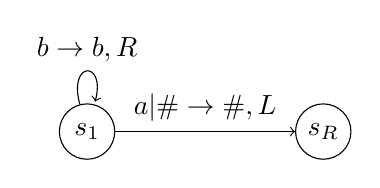
\begin{tikzpicture}
            \node[circle, draw=black, fill=white, inner sep=0pt, minimum size=20pt] (s1) at (0, 0) {$s_1$};
            \node[circle, draw=black, fill=white, inner sep=0pt, minimum size=20pt] (sR) at (3, 0) {$s_R$};

            \draw[->] (s1) -- node[above] {$a | \# \to \#, L$} (sR);
            \draw[->] (s1) edge[loop above] node[above] {$b \to b, R$} (s1);
        \end{tikzpicture}
        \caption{The sub-TM of the given Turing Machine complete module.}
    \end{figure}
    \end{example}
    \begin{remark}
        In the example above, we consider the state $s_1$ to be the \emph{corresponding state} of the module. For every complete module, there is precisely one corresponding state.
    \end{remark}

    Now, we can define complete programs.
    \begin{definition}
        Let $P$ be a TML program. We say that $P$ is \emph{complete} if it is composed of one or more complete modules. We also require every \textit{goto} command in a complete block to refer to an existing module.
    \end{definition}
    \begin{remark}
        The second condition (called \emph{valid reference}) is required for any TML program.
    \end{remark}
    \begin{remark}
        In general, a complete program is not composed of a single complete module. We will see later that a relatively simple module can be broken down into a couple of complete modules, each of which refer to each other.
    \end{remark}
    Every module in the program can be converted to a state, along with directed edges to other states. If the program is complete, then we ensure that the states connect to form a valid TM.
    \begin{example}
        Consider the following complete program.
\begin{lstlisting}[language=TML]
alphabet = {"a", "b"}
module isDivTwo {
    switch tapehead {
        while 0 {
            changeto 0
            move right
        } while 1 {
            changeto 1
            move right
        } if blank {
            changeto blank
            move left
            goto isDivTwoCheck
        }
    }
}
module isDivTwoCheck {
    switch tapehead {
        if 0 {
            changeto 0
            move left
            accept
        } if 1, blank {
            changeto blank
            move left
            reject
        }
    }
}
\end{lstlisting}
    Then, the corresponding TM is the following:
    \begin{figure}[H]
        \centering
        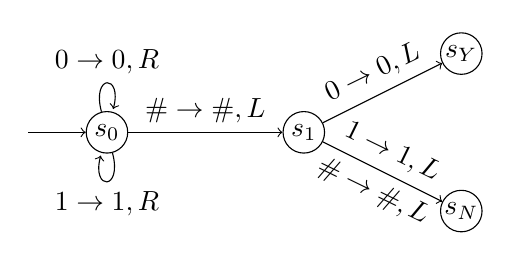
\begin{tikzpicture}
            \node[circle, draw=black, fill=white, inner sep=0pt, minimum size=15pt] (s0) at (0, 0) {$s_0$};
            \node[circle, draw=black, fill=white, inner sep=0pt, minimum size=15pt] (s1) at (2.5, 0) {$s_1$};
            \node[circle, draw=black, fill=white, inner sep=0pt, minimum size=15pt] (sY) at (4.5, 1) {$s_Y$};
            \node[circle, draw=black, fill=white, inner sep=0pt, minimum size=15pt] (sN) at (4.5, -1) {$s_N$};
            
            \draw[->] (-1, 0) -- (s0);
            \draw[->] (s0) edge[loop above] node[above] {$0 \to 0, R$} (s0);
            \draw[->] (s0) edge[loop below] node[below] {$1 \to 1, R$} (s0);
            \draw[->] (s0) -- node[above] {$\# \to \#, L$} (s1);
            \draw[->] (s1) -- node[above, rotate=26] {$0 \to 0, L$} (sY);
            \draw[->] (s1) -- node[above, rotate=-26] {$1 \to 1, L$} node[below, rotate=-26] {$\# \to \#, L$} (sN);
        \end{tikzpicture}
        \caption{The TM of the given TML program. The state $s_0$ corresponds to the module \texttt{isDivTwo} and the state $s_1$ corresponds to the module \texttt{isDivTwoCheck}.}
    \end{figure}
    \end{example}
    \begin{remark}
        In the example above, we converted a complete TML program into a TM. It is equally possible to convert a TM into a complete TML program.
    \end{remark}
    \begin{example}
        Consider the following TM:
        \begin{figure}[H]
            \centering
            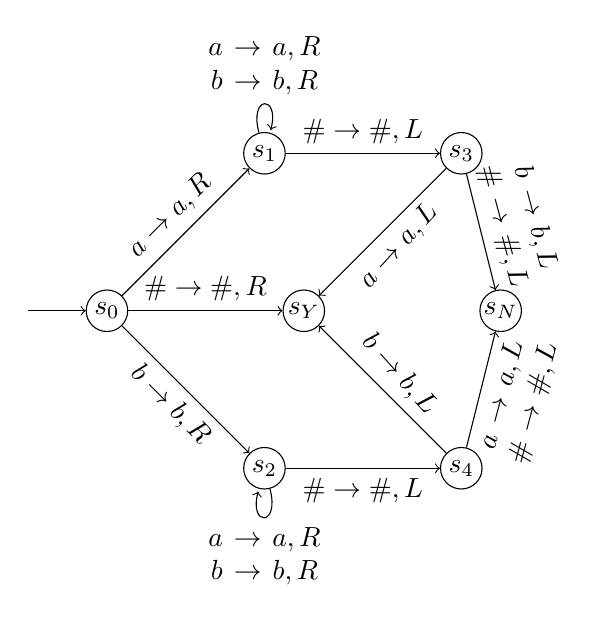
\begin{tikzpicture}
                \node[circle, draw=black, fill=white, inner sep=0pt, minimum size=15pt] (s0) at (0, 0) {$s_0$};
                \node[circle, draw=black, fill=white, inner sep=0pt, minimum size=15pt] (s1) at (2, 2) {$s_1$};
                \node[circle, draw=black, fill=white, inner sep=0pt, minimum size=15pt] (s2) at (2, -2) {$s_2$};
                \node[circle, draw=black, fill=white, inner sep=0pt, minimum size=15pt] (s3) at (4.5, 2) {$s_3$};
                \node[circle, draw=black, fill=white, inner sep=0pt, minimum size=15pt] (s4) at (4.5, -2) {$s_4$};
                \node[circle, draw=black, fill=white, inner sep=0pt, minimum size=15pt] (sY) at (2.5, 0) {$s_Y$};
                \node[circle, draw=black, fill=white, inner sep=0pt, minimum size=15pt] (sN) at (5, 0) {$s_N$};
                
                \draw[->] (-1, 0) -- (s0);
                \draw[->] (s0) -- node[above, rotate=45] {$a \to a, R$} (s1);
                \draw[->] (s0) -- node[below, rotate=-45] {$b \to b, R$} (s2);
                \draw[->] (s0) -- node[above] {$\# \to \#, R$} (sY);
                \draw[->] (s1) edge[loop above] node[above, text width=2cm, align=center] {$a \to a, R$ $b \to b, R$} (s1);
                \draw[->] (s2) edge[loop below] node[below, text width=2cm, align=center] {$a \to a, R$ $b \to b, R$} (s2);
                \draw[->] (s1) -- node[above] {$\# \to \#, L$} (s3);
                \draw[->] (s2) -- node[below] {$\# \to \#, L$} (s4);
                \draw[->] (s3) -- node[above, rotate=-75, text width=2cm, align=center] {$b \to b, L$ $\# \to \#, L$} (sN);
                \draw[->] (s4) -- node[below, rotate=75, text width=2cm, align=center] {$a \to a, L$ $\# \to \#, L$} (sN);
                \draw[->] (s3) -- node[below, rotate=48] {$a \to a, L$} (sY);
                \draw[->] (s4) -- node[above, rotate=-48] {$b \to b, L$} (sY);
            \end{tikzpicture}
            \caption{A Turing machine}
        \end{figure}
        \noindent Then, its corresponding TML program is:
\begin{lstlisting}[language=TML]
alphabet = {"a", "b"}
module startsAndEndsSame {
    switch tapehead {
        if blank {
            accept
        } if a {
            changeto a
            move right
            goto startsAndEndsSameMoveA
        } if b {
            changeto b
            move right
            goto startsAndEndsSameMoveB
        }
    }
}
module startsAndEndsSameMoveA {
    switch tapehead {
        while a {
            changeto a
            move right
        } while b {
            changeto b
            move right
        } if blank {
            changeto blank
            move left
            goto startsAndEndsSameCheckA
        }
    }
}
module startsAndEndsSameCheckA {
    switch tapehead {
        if a {
            changeto a
            move left
            accept
        } if b {
            changeto b
            move left
            reject
        } if blank {
            changeto blank
            move left
            reject
        }
    }
}
module startsAndEndsSameMoveB {
    switch tapehead {
        while a {
            changeto a
            move right
        } while b {
            changeto b
            move right
        } if blank {
            changeto blank
            move left
            goto startsAndEndsSameCheckB
        }
    }
}
module startsAndEndsSameCheckB {
    switch tapehead {
        if a {
            changeto a
            move left
            reject
        } if b {
            changeto b
            move left
            accept
        } if blank {
            changeto blank
            move left
            reject
        }
    }
}
\end{lstlisting}
    This is a complete program since TMs always include the required commands corresponding to \textit{if} and \textit{while} commands.
    \end{example}
    \begin{remark}
        Although a TML program need not be complete, any valid TML program is equivalent to a complete one. So, a TML program that is not be complete is just a compact representation of its complete version.
    \end{remark}

\end{document}